\chapter{SLAM}

\paragraph*{}
This chapter details the progress on implementing simple SLAM as per the Gantt chart. 

\paragraph*{}
The primary goal of this project was to implement SLAM for the TurtleBot3 in the Webots simulation environment. Here’s a summary of how SLAM was implemented step-by-step:

\paragraph*{}
We started by importing the TurtleBot3Burger model into the Webots simulation. TurtleBot3 was chosen for its compatibility with LIDAR sensors and wheel encoders, which are essential for SLAM. Additionally, we configured the simulation to include LIDAR for obstacle detection and positional sensors (encoders) to track the robot’s wheel rotations.

\paragraph*{}
The motors controlling the TurtleBot’s left and right wheels were set up to allow the robot to move forward and rotate. These motors were managed by adjusting their velocity and setting their positions to infinity, which allows continuous rotation. Motor control is essential to ensure the robot can explore the environment and collect data for mapping.

\paragraph*{}
The TurtleBot3 was equipped with a LIDAR sensor to scan its surroundings and detect obstacles. The LIDAR provides 360° range data, which is essential for building an occupancy grid map. The wheel encoders (PositionSensors) track the movement of each wheel, allowing us to calculate the robot’s odometry (its position and orientation in space).

\paragraph*{}
To track the TurtleBot’s position in the simulated environment, we used the encoder readings from the wheels to calculate the robot’s change in position ($x$, $y$) and orientation ($\theta$). This was done by using differential drive kinematics, which calculates the distance travelled by each wheel and translates that into movement and rotation of the robot.

\paragraph*{}
The SLAM algorithm consists of two primary components: localization (tracking the robot’s position) and mapping (creating an occupancy grid map based on LIDAR data).

\begin{itemize}
    \item \textbf{Mapping}: The LIDAR data, which measures distances to nearby obstacles, was used to update a 2D occupancy grid map. The robot’s position and orientation are used to convert the LIDAR data into world coordinates, which are then translated into the corresponding grid cells. Each cell in the grid can be marked as either free space or occupied (by an obstacle).
    \item \textbf{Localization}: The odometry data (robot position and orientation) was continuously updated based on the encoder values, ensuring that the TurtleBot accurately tracked its position relative to the environment.
\end{itemize}

\paragraph*{}
An occupancy grid map was created to represent the environment. This map is a 2D array where each cell represents a small portion of the environment. If a LIDAR beam detects an obstacle in a particular direction, the corresponding cell in the map is marked as occupied. If no obstacle is detected, the cell is left free. The map is updated in real-time as the TurtleBot moves and scans its surroundings. A periodic printing function was also implemented to visualise the progress of the SLAM algorithm.

\paragraph*{}
One challenge was ensuring that the map updates properly with every step of the robot’s movement. To handle this, we implemented periodic map printing and added debug messages to track the progress of the algorithm. Additionally, the proper setup of sensors, particularly LIDAR and encoders, was critical to ensuring accurate mapping and localization.

\paragraph*{}
The implementation of SLAM in Webots using TurtleBot3 has successfully allowed us to map an environment while localizing the robot within that map. By integrating LIDAR and encoder data, we were able to track the robot’s movement and continuously update the environment map in real time. TurtleBot3 provided an ideal platform due to its modular design and compatibility with SLAM-related sensors. Moving forward, further refinement of the SLAM algorithm, such as enhancing obstacle detection or improving localization accuracy, could make the system even more robust.

\begin{itemize}
    \item \textbf{Improved Mapping Resolution}: Experiment with different map resolutions to enhance the detail of the mapped environment.
    \item \textbf{Obstacle Avoidance}: Integrate path planning and obstacle avoidance based on the SLAM map.
    \item \textbf{Integration with ROS}: Explore connecting the TurtleBot3 to ROS for more advanced SLAM algorithms and leveraging existing ROS packages for autonomous navigation.
\end{itemize}

\begin{figure}
    \centering
    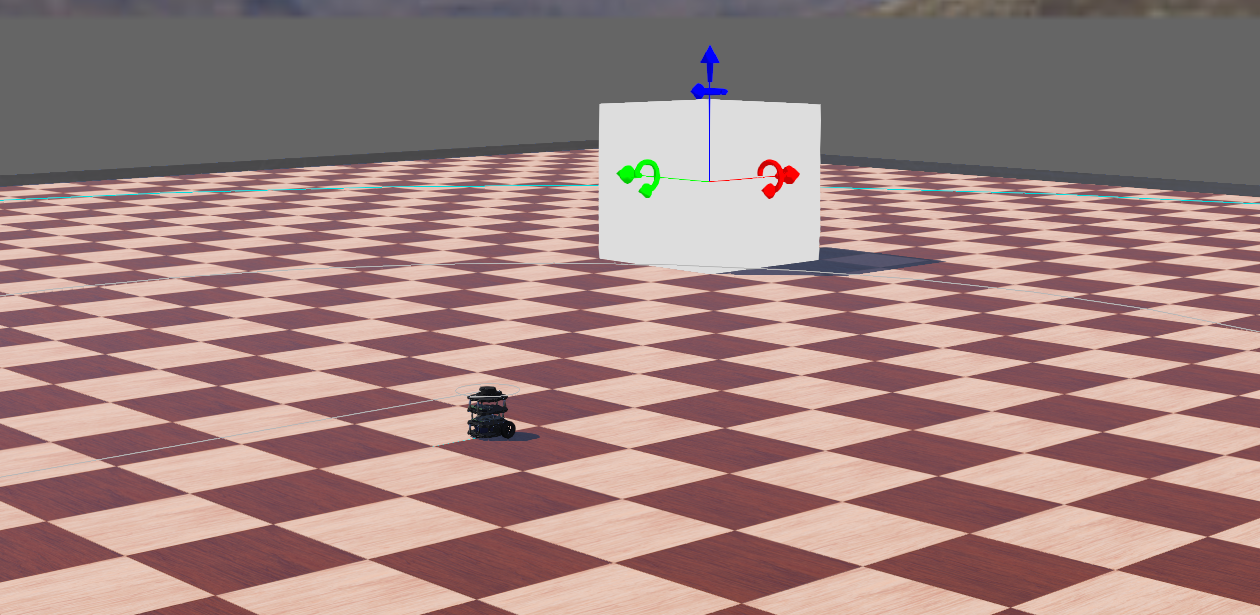
\includegraphics[width=1\linewidth]{assets/images/slam/environment.png}
    \caption{SLAM Environment}
    \label{fig:slam_environment}
\end{figure}

\begin{figure}
    \centering
    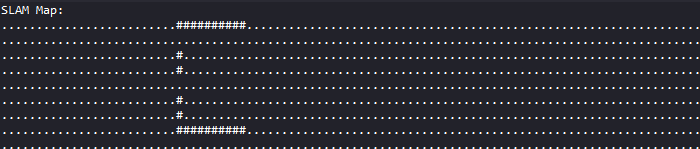
\includegraphics[width=1\linewidth]{assets/images/slam/output.png}
    \caption{Output in the Terminal}
    \label{fig:slam_output}
\end{figure}
